% Formatvorlage f\"{u}r das Seminar "Robotik und Prozessinformatik"
%
% Technische Universitaet Braunschweig
% Institut fuer Robotik und Prozessinformatik
% Muehlenpfordtstrasse 23
% D-38106 Braunschweig
% GERMANY
%
% http://www.cs.tu-bs.de/rob
%
% Torsten Kroeger, t.kroeger@tu-bs.de
%
% April 2007
%
%

\documentclass[german, 10pt]{report}
\usepackage{a4}
\usepackage{doku}
\usepackage{german}
\usepackage{longtable}
%\usepackage[draft]{graphicx}
\usepackage{graphicx}
\usepackage{graphics}
\usepackage{epstopdf} %converts eps to pdf while using pdflatex
\usepackage{bbm}
\usepackage[dvips]{epsfig}
\usepackage{ngerman}
\usepackage{nomencl}


% #######################################################################
% Titelseite
% #######################################################################


\begin{document}
\large \selectlanguage{ngerman}
\pagenumbering{roman}
\begin{titlepage}
    \setcounter{page}{1}
    \let\footnotesize\small
    \let\footnoterule\relax
    \headsep 1.5cm
    \vskip -4cm
    \centerline{\Huge\bf Technische Universit\"{a}t Braunschweig}
    \vskip 3.4cm
    \begin{center}
        \begin{minipage}[t][7cm][c]{13.5cm}
            \begin{center}
                {\large{Seminar \glqq Fortschritte in der Robotik\grqq\\}\par}
                \vskip 0.5cm
                {\LARGE\bf {T-i-t-e-l---d-e-s---V-o-r-t-r-a-g-s}}
                \vskip 0.5cm
                {\Large\bf N-a-m-e---d-e-s---T-e-i-l-n-e-h-m-e-r-s}
                \vskip 0.25cm
                {\large\bf Betreuer: N-a-m-e---d-e-s---B-e-t-r-e-u-e-r-s}
                \vskip 0.75cm
                {\large\bf{D-a-t-u-m---d-e-r---A-b-g-a-b-e}\par}
            \end{center}
        \end{minipage}
    \end{center}
    \vskip 2.0cm
    \begin{figure}[h]
        \begin{center}
            
\includegraphics{TU-Logo.eps}
        \end{center}
    \end{figure}
    \vskip 1cm
    \centerline{\LARGE\bf Institut f\"{u}r Robotik und Prozessinformatik}
    \vskip 1cm
    \centerline{\LARGE\bf Prof.~Dr.~F.~Wahl}




\end{titlepage}
\setcounter{footnote}{0}
\setcounter{totalnumber}{8}

% #######################################################################
% Inhaltsverzeichnis
% #######################################################################
\thispagestyle{empty}
\newpage

\tableofcontents \thispagestyle{headings}
\setlength{\baselineskip}{3ex}


% #######################################################################
% Dokument
% #######################################################################


\chapter{Einleitung}
\pagenumbering{arabic}\label{C_Einleitung}Diese Arbeit ist
Bestandteil des Seminars \glqq Robotik und Prozessinformatik\grqq \
der Carl-Friedrich-Gau{\ss}-Fakult\"{a}t an der Technischen Universit\"{a}t
Braunschweig. Das Thema...


% #######################################################################
\section{Beispiel f\"{u}r eine Abbildung}
\label{S_AbbBeispiel}Wie man Abb.~\ref{F_BeispielBild} entnehmen
kann...

\begin{figure}
    \centering
    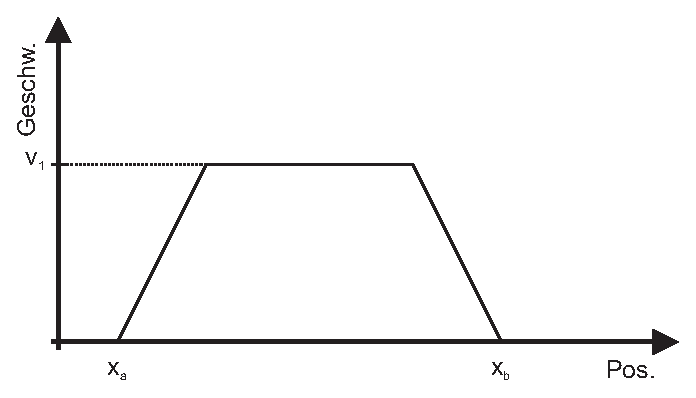
\includegraphics[width=0.6\linewidth]{BeispielBild.eps}
    \caption{\label{F_BeispielBild}Beispielbildunterschrift: Trajektorienverlauf f\"{u}r eine H\"{o}chstgeschwindigkeit $v_1$ um von Position $x_a$ nach $x_b$ zu gelangen.}
\end{figure}


% #######################################################################
\section{Ein einfaches Unterkapitel mit einer Beispieltabelle}
\label{S_Unterkapitel}Aus Tab.~\ref{T_BeispielTabelle} kann man
entnehmen, dass...

\begin{table}[h]
    \centering
    \begin{tabular}{|c|c|c|c|c|}\hline
        &$m$ & $c_{x}$  & $c_{y}$ & $c_{z}$\\\hline
        Mittelwert & $56.5g$ & $-1.7mm$ & $0.4mm$ & $10.3mm$\\\hline
        Varianz & $0.017g^2$ & $0.0067mm^2$ & $0.0079mm^2$ & $0.0098mm^2$\\\hline
    \end{tabular}
    \caption{\label{T_BeispielTabelle}Unterschrift f\"{u}r eine Beispieltabelle.}
\end{table}


% #######################################################################
\chapter{Beispielkapitel}
\label{C_Kapitel}Dieses Kapitel er\"{o}rtert...


% #######################################################################
\section{Darstellung eines Bildes}
\label{S_Bild}Ein Bild besteht aus...


% #######################################################################
\subsection{Darstellung einer Bildzeile}
\label{S_Bildzeile}Eine einzelne Bildzeile eines gegebenen Bildes
wird...


% #######################################################################
\subsubsection{Darstellung eines Bildpixels}
\label{S_Bildpixels}Bildpunkte (Pixel) werden...



% #######################################################################
\section{Beispiel f\"{u}r eine Formel}
\label{S_Formel}Fasst man Kap.~\ref{S_Unterkapitel} und \ref{S_Bild}
zusammen, ergibt sich $b$ aus Gl.~\ref{E_Bild}:

\begin{equation}
    \left.
    b:\{0,\dots,511\}\times\{0,\dots,255\}\longrightarrow\{0,1\}\mbox{
    mit }\left\{
    \begin{array}{rcl}
        b(x,y)=1&\Leftrightarrow & \mbox{Pixel $(x,y)$ schwarz}\\
        b(x,y)=0\normalsize&\Leftrightarrow & \mbox{Pixel $(x,y)$ wei{\ss}}\\
    \end{array}
    \right.\right.\label{E_Bild}
\end{equation}


% #######################################################################
\chapter{Zusammenfassung}
\label{C_Zusammenfassung}Zusammenfassend l\"{a}sst sich festhalten,
dass...


% #######################################################################
\section{Beispiel f\"{u}r eine Aufz\"{a}hlung}
\label{S_Aufzaehlung}Im Folgenden sei
\begin{itemize}
    \item $^{S}p_{a}$, die Position von Objekt $a$ bez\"{u}glich System $S$
    \item $^{\Lambda}p_{b}$, die Position von Objekt $b$ bez\"{u}glich der Basis
    $\Lambda$.\\
\end{itemize}


% #######################################################################
\section{Beispiel f\"{u}r eine Nummerierung}
\label{S_Nummerierung}Anleitung zum Herstellen von Tapetenkleister:

\begin{enumerate}
    \item Sie nehmen einen Eimer und f\"{u}llen diesen mit f\"{u}nf Liter
    Wasser.
    \item Den Inhalt der Packung sch\"{u}tten Sie unter st\"{a}ndigem R\"{u}hren in die
    Fl\"{u}ssigkeit.
    \item ...\\
\end{enumerate}



% #######################################################################
\section{Beispiele f\"{u}r Zitate}
\label{S_ZitatBeispiele}{\bf Beispiel f\"{u}r ein Zitat eines
Zeitschriftenartikels:} Amarasinghe et.~al.~haben in
\cite{Amarasinghe:07} bewiesen, dass...\\

{\bf Beispiel f\"{u}r ein Zitat eines Buches:} Nimmt man
\cite{Baeten:04} als Grundlage f\"{u}r...\\

{\bf Beispiel f\"{u}r ein Zitat einer Internetquelle:} Auch in \cite{Autosar:05} wurde schon demonstriert, dass...\\

{\bf Beispiel f\"{u}r ein Zitat aus einem Tagungsband:} Anhand des
Einsatzes von Echtzeitsystemen f\"{u}r die Generierung von
Bewegungsprofilen wird in \cite{Benhabib:04} beispielhaft er\"{o}rtert,
dass...\\

{\bf Beispiel f\"{u}r ein Zitat aus einer Dissertation:} Wie schon
Bruyninckx im Jahr 1995 gezeigt hat, ist der TF-Formalismus eine
wichtige Methode im Bereich der Robotik \cite{Bruyninckx:95}.\\

% #######################################################################
% Anhang
% #######################################################################

\begin{appendix}

% #######################################################################
\chapter{Beschreibung der einzelnen mathematischen Methoden}
\label{C_MathMethoden} In diesem Abschnitt werden die verschiedenen
mathematischen Vorgehensweisen...


% #######################################################################
\section{Ansatz nach Benhabib}
Der Kern des Ansatzes von Benhabib \cite{Benhabib:04} ist...


% #######################################################################
\chapter{Noch ein Beispielanhang}
\label{C_BeispielAnhang}


\end{appendix}

% #######################################################################
% Abbildungsverzeichnis
% #######################################################################

\addcontentsline{toc}{chapter}{Abbildungsverzeichnis} \listoffigures

% #######################################################################
% Tabellenverzeichnis
% #######################################################################

\newpage
\addcontentsline{toc}{chapter}{Tabellenverzeichnis} \listoftables

% #######################################################################
% Literaturverzeichnis
% #######################################################################

\newpage
\addcontentsline{toc}{chapter}{Literaturverzeichnis}
\newpage
\bibliographystyle{unsrtdin}
\bibliography{./LiteraturVorlage}

\end{document}
